\chapter{Propiedades geométricas, de masa y de rigidez}
\label{ch:propiedades}
\section{Geometría, densidad y medida de integración}
Una propiedad másica no se identifica únicamente por su valor: debe conocerse el dominio sobre el que se integra, el punto respecto del cual se calcula y la base utilizada para sus componentes. En una viga, las propiedades por unidad de longitud se definen sobre la sección material de referencia $A_0(S)$. Para una sección recta se usa el vector transversal $\vct\zeta=\xi_2\vct D_2+\xi_3\vct D_3$. La densidad de referencia $\rho_0$ se mide en $\mathrm{kg/m^3}$.

Se adopta localmente la medida prismática $\dd V_0=\dd A_0\dd S$, válida para el elemento recto empleado en la discretización. En una parametrización curva general, el determinante del transformación geométrica interviene en esta medida y no debe omitirse. La reducción a propiedades por longitud que sigue corresponde a esa aproximación local recta.

\section{Momentos geométricos de la sección}
El área, su primer momento y su centro geométrico son
\begin{equation}
 A=\int_{A_0}\dd A_0,\qquad
 \vct a_A=\int_{A_0}\vct\zeta\,\dd A_0,\qquad
 \vct c_A=\frac{\vct a_A}{A}.
\end{equation}
Con $\vct\eta_A=\vct\zeta-\vct c_A$, el tensor de segundos momentos geométricos se define por
\begin{equation}
 \ten S_A=\int_{A_0}\vct\eta_A\otimes\vct\eta_A\,\dd A_0,
 \qquad
 \ten I_A=\operatorname{tr}(\ten S_A)\Id-\ten S_A.
 \label{eq:area_tensor}
\end{equation}
Los tensores $\ten S_A$ e $\ten I_A$ tienen dimensión $\mathrm{m^4}$, son simétricos y describen la distribución de área, no de masa. El segundo es conveniente para relacionar un eje de giro con el segundo momento respecto a ese eje. En la base de sección con eje longitudinal $\vct D_1$, las coordenadas de $\vct\eta_A$ son $(0,y,z)$ y
\begin{equation}
 [\ten I_A]=
 \begin{bmatrix}
 \int(y^2+z^2)\dd A_0&0&0\\
 0&\int z^2\dd A_0&-\int yz\dd A_0\\
 0&-\int yz\dd A_0&\int y^2\dd A_0
 \end{bmatrix}.
\end{equation}
Así, $I_2=\int z^2\dd A_0$ e $I_3=\int y^2\dd A_0$. Un producto $\int yz\dd A_0$ no se introduce con signo positivo en las entradas fuera de la diagonal del tensor de inercia geométrico. Las direcciones principales diagonalizan su bloque transversal.

La constante torsional de Saint-Venant se denota $J_t$ y también tiene unidades de $\mathrm{m^4}$. No se identifica en general con $I_2+I_3$. Esta igualdad es válida para secciones circulares, pero no para una sección aerodinámica genérica: la distribución de tensiones de torsión depende del alabeo. Usar un momento polar de área como constante torsional sin esa justificación modifica la rigidez del modelo.

La figura~\ref{fig:centros} distingue el punto de referencia $O_s$, el centro de área $C_A$ y el centro de masa seccional $C_m$. Esta distinción permite definir a continuación las propiedades de masa sin suponer que los tres puntos coinciden.

\begin{figure}[htbp]
\centering
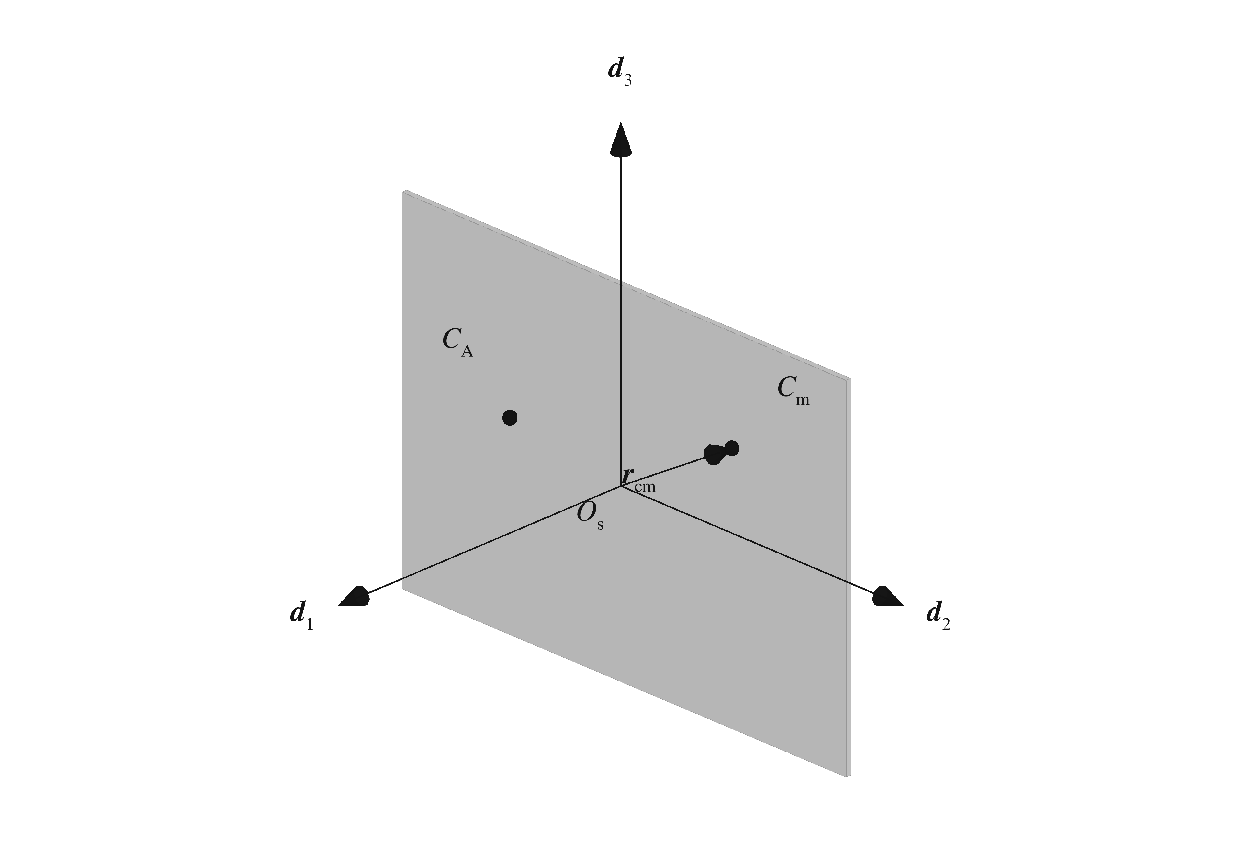
\includegraphics[width=.96\linewidth,height=.40\textheight,keepaspectratio]{figures/tecplot/concept_centros.pdf}
\caption[Punto de referencia y centros seccionales]{Sección con espesor ilustrativo y triedro completo: punto de referencia $O_s$, centro de área $C_A$ y centro de masa $C_m$. $\vct r_{cm}$ localiza el centro de masa respecto de $O_s$. Las posiciones se eligen para distinguir las definiciones; no corresponden a una sección medida.}\label{fig:centros}
\end{figure}

\section{Masa por longitud y tensor de inercia seccional}
La masa por longitud y el primer momento másico son
\begin{equation}
 \mu(S)=\int_{A_0}\rho_0\,\dd A_0,\qquad
 \vct h_m(S)=\int_{A_0}\rho_0\vct\zeta\,\dd A_0,\qquad
 \vct c_m=\frac{\vct h_m}{\mu}.
\end{equation}
El centro de masa depende de la densidad. Si esta es constante en la sección, $\vct c_m=\vct c_A$; una pala compuesta no cumple necesariamente esta condición. La inercia por longitud respecto de $C_m$, con $\vct\eta_m=\vct\zeta-\vct c_m$, es
\begin{equation}
 \ten j_C=\int_{A_0}\rho_0
 \left[(\vct\eta_m\cdot\vct\eta_m)\Id-\vct\eta_m\otimes\vct\eta_m\right]\dd A_0.
 \label{eq:jC}
\end{equation}
Sus unidades son $\mathrm{kg\,m}$, no $\mathrm{kg\,m^2}$. La integración posterior sobre $S$ incorpora la dimensión de longitud restante. Para cualquier vector angular $\vct\omega$,
\begin{equation}
 \vct\omega\cdot\ten j_C\vct\omega
 =\int_{A_0}\rho_0\|\vct\omega\times\vct\eta_m\|^2\dd A_0\geq0.
\end{equation}
Esta identidad muestra directamente su significado físico: cuantifica la energía cinética asociada al movimiento rotacional de la distribución de masa seccional.

En una sección plana, $j_1=j_2+j_3$ respecto del mismo centro y en una base ortonormal con eje 1 normal a la sección. No es una condición que se imponga a un cuerpo tridimensional arbitrario. Si $\rho_0$ es constante y los centros coinciden, $\ten j_C=\rho_0\ten I_A$.

El traslado al punto $O_s$ se deduce al introducir $\vct\zeta=\vct c_m+\vct\eta_m$ en la integral. Los términos lineales desaparecen porque $\int\rho_0\vct\eta_m\dd A_0=\vct0$. Resulta
\begin{equation}
 \ten j_O=\ten j_C+\mu\left[(\vct c_m\cdot\vct c_m)\Id-\vct c_m\otimes\vct c_m\right]
 =\ten j_C-\mu\sk{c_m}^{2}.
 \label{eq:steiner}
\end{equation}
El signo menos en la segunda forma no implica una disminución de inercia: $-\sk{c_m}^{2}$ es semidefinida positiva. Ambas expresiones son la misma identidad de ejes paralelos.

La figura~\ref{fig:masa-seccional} permite reconstruir la integral sin confundir los puntos de referencia. El vector material desde $O_s$ hasta una partícula es $\vct\zeta=\vct c_m+\vct\eta_m$. La integración respecto de $C_m$ utiliza $\vct\eta_m$; el traslado a $O_s$ utiliza la excentricidad $\vct c_m$. Por ello la identidad de ejes paralelos no sustituye al cambio de base del tensor.
\begin{figure}[htbp]
\centering
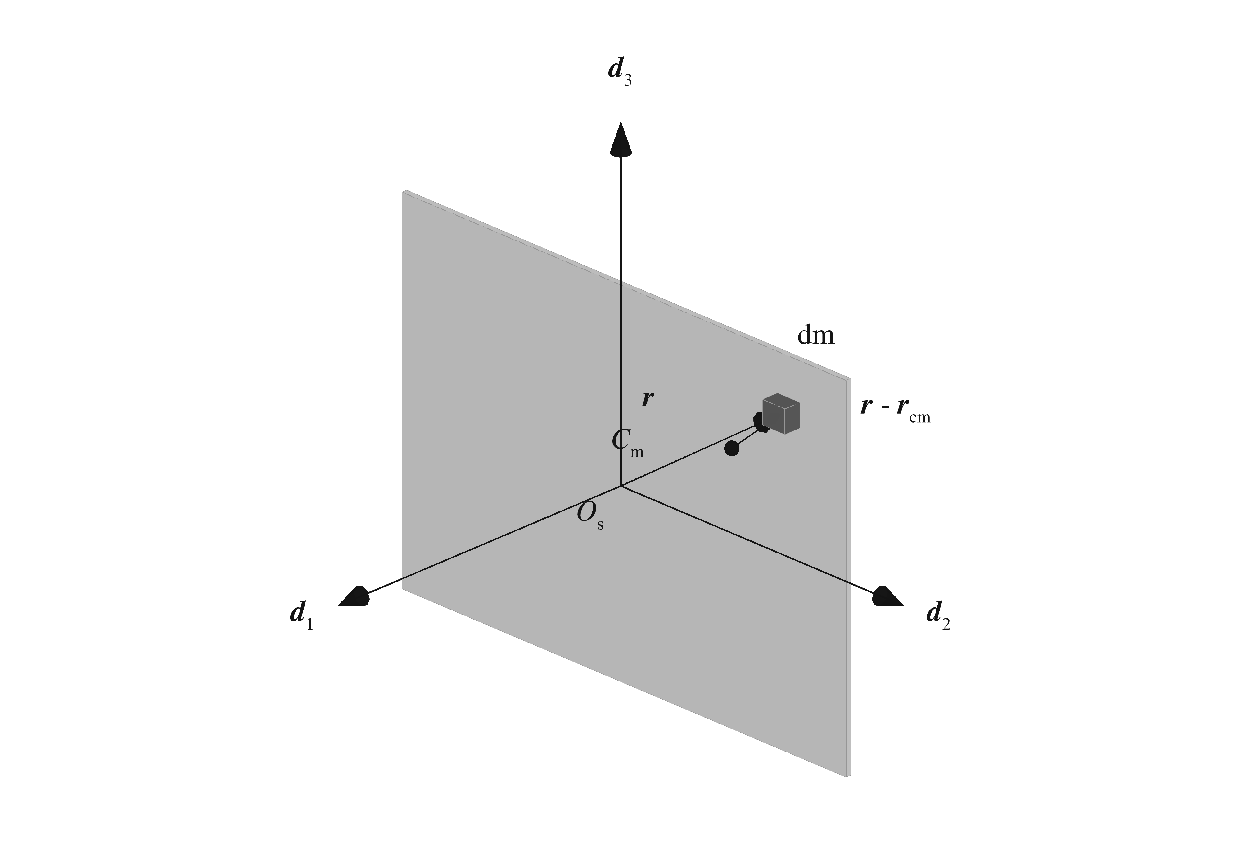
\includegraphics[width=.96\linewidth,height=.40\textheight,keepaspectratio]{figures/tecplot/concept_masa-seccional.pdf}
\caption[Geometría de la integración de masa]{Geometría de la integración de masa en una sección. $\vct r$ sitúa el elemento $\dd m$ respecto de $O_s$ y $\vct r-\vct r_{cm}$ lo sitúa respecto del centro de masa $C_m$. El espesor de la superficie y el tamaño del elemento de masa son ilustrativos.}\label{fig:masa-seccional}
\end{figure}

\section{Cuerpos rígidos tridimensionales}
Para una góndola o un cubo se integra sobre su volumen de referencia $V_0$:
\begin{align}
 m&=\int_{V_0}\rho_0\dd V_0,&
 \vct X_C&=\frac1m\int_{V_0}\rho_0\vct X\dd V_0,\\
 \ten J_C&=\int_{V_0}\rho_0\left[\|\vct X-\vct X_C\|^2\Id
 -(\vct X-\vct X_C)\otimes(\vct X-\vct X_C)\right]\dd V_0.
\end{align}
Ahora $m$ se expresa en $\mathrm{kg}$ y $\ten J_C$ en $\mathrm{kg\,m^2}$. La diferencia de mayúscula entre $\ten J_C$ y $\ten j_C$ distingue cantidades integradas en un volumen y cantidades por longitud, respectivamente.

Las propiedades obtenidas de un modelo geométrico tridimensional se expresan respecto de un origen, una base y un sistema de unidades determinados. El traslado al punto de referencia del cuerpo utiliza la identidad~\eqref{eq:steiner} con $\mu$ sustituido por $m$. El cambio de base del tensor completo se realiza mediante
\begin{equation}
 [\ten J_C]^A={}^A Q_B[\ten J_C]^B({}^A Q_B)^\tr.
\end{equation}
Primero se declara dónde está el centro y en qué base se conoce el tensor; luego se rota y traslada con esas mismas convenciones. Transformar solo tres valores diagonales ignora los productos de inercia generados por el cambio de orientación.

Para una representación mediante masas puntuales, la integral se aproxima por
\begin{equation}
 m\simeq\sum_k m_k,\quad
 \vct X_C\simeq m^{-1}\sum_k m_k\vct X_k,\quad
 \ten J_C\simeq\sum_k m_k\left[\|\vct r_k\|^2\Id-\vct r_k\otimes\vct r_k\right].
\end{equation}
Si cada componente tiene extensión finita, también debe sumarse su propio tensor centroidal rotado. Reemplazar cada componente por una masa puntual omite esa contribución. Una masa total por sí sola no permite reconstruir un tensor de inercia.

\section{Energía cinética y tensor de inercia de un cuerpo rígido}
\subsection{Posición de una partícula y centro de masa}
Considérese un cuerpo rígido con un punto de referencia $O$, solidario con el cuerpo, y centro de masa $C$. Para una partícula $P$ se definen los vectores $\vct r=\overrightarrow{OP}$, $\vct c=\overrightarrow{OC}$ y $\vct\rho=\overrightarrow{CP}$. Todos se consideran en la configuración actual y cumplen
\begin{equation}
 \vct r=\vct c+\vct\rho,\qquad
 \vct x_P=\vct x_O+\vct r=\vct x_C+\vct\rho.
 \label{eq:posicion-centromasa}
\end{equation}
Las componentes de $\vct r$ en una base solidaria permanecen constantes. En una base inercial varían con la orientación del cuerpo, por lo que el teorema de transporte proporciona
\begin{equation}
 \vct v_P=\vct v_O+\vct\omega\times\vct r
         =\vct v_C+\vct\omega\times\vct\rho,\qquad
 \vct v_C=\vct v_O+\vct\omega\times\vct c.
 \label{eq:velocidad-rigido-centro}
\end{equation}
La velocidad angular $\vct\omega$ es común a todas las partículas; sus velocidades lineales dependen de la distancia al eje instantáneo de rotación.

En la figura~\ref{fig:rigido-centro}, las posiciones absolutas y los vectores relativos se dibujan por separado para identificar las contribuciones a la velocidad de una partícula.

\begin{figure}[htbp]
\centering
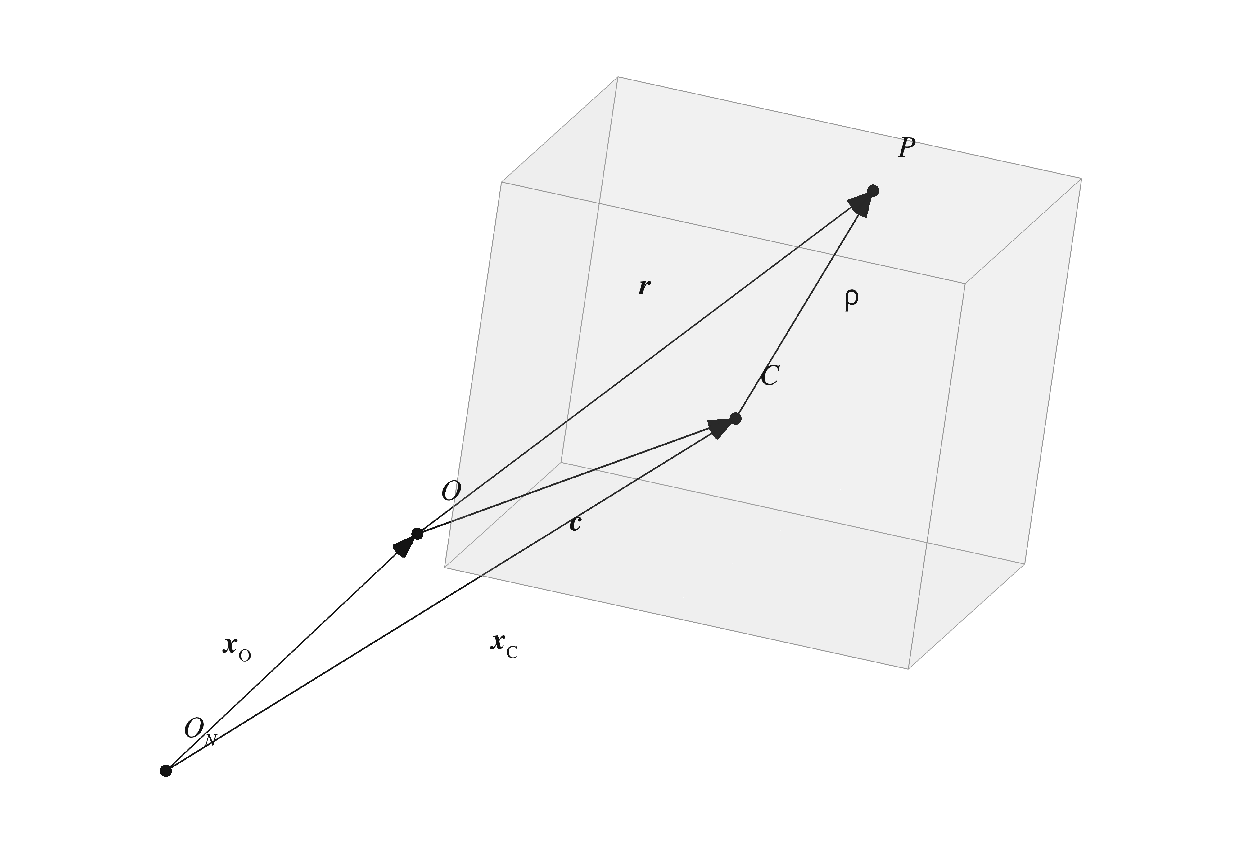
\includegraphics[width=.96\linewidth,height=.40\textheight,keepaspectratio]{figures/tecplot/concept_rigido-centro.pdf}
\caption[Posición de una partícula de cuerpo rígido]{Posiciones absolutas y relativas de una partícula de cuerpo rígido. Se cumple $\vct x_P=\vct x_O+\vct r=\vct x_C+\vct\rho$ y $\vct r=\vct c+\vct\rho$. La envolvente transparente sitúa el cuerpo y permite seguir los vectores desde el origen inercial $O_N$.}\label{fig:rigido-centro}
\end{figure}

Por definición del centro de masa,
\begin{equation}
 m\vct c=\int_{\mathcal B}\vct r\,\dd m,\qquad
 \int_{\mathcal B}\vct\rho\,\dd m
 =\int_{\mathcal B}(\vct r-\vct c)\,\dd m=\vct0.
 \label{eq:primer-momento-nulo}
\end{equation}
La medida $\dd m=\rho_0\dd V_0$ permanece constante durante el movimiento. Por ello la integración puede realizarse sobre la configuración de referencia, aunque los vectores se expresen en la configuración actual.

\subsection{Separación de traslación y rotación}
La energía cinética se obtiene integrando la contribución de cada partícula. Al sustituir la segunda forma de \eqref{eq:velocidad-rigido-centro},
\begin{align}
 T&=\frac12\int_{\mathcal B}\vct v_P\cdot\vct v_P\,\dd m\nonumber\\
 &=\frac12m\,\vct v_C\cdot\vct v_C
 +\vct v_C\cdot\left(\vct\omega\times
             \int_{\mathcal B}\vct\rho\,\dd m\right)
 +\frac12\int_{\mathcal B}\|\vct\omega\times\vct\rho\|^2\,\dd m.
 \label{eq:T-desarrollo}
\end{align}
El término cruzado es nulo por \eqref{eq:primer-momento-nulo}. Para el último término se emplea la identidad
\begin{equation}
 \|\vct\omega\times\vct\rho\|^2
 =\|\vct\omega\|^2\|\vct\rho\|^2-(\vct\omega\cdot\vct\rho)^2
 =\vct\omega\cdot
   \left[(\vct\rho\cdot\vct\rho)\Id-\vct\rho\otimes\vct\rho\right]\vct\omega.
\end{equation}
Así aparece el tensor de inercia respecto del centro de masa,
\begin{equation}
 \ten J_C=\int_{\mathcal B}
       \left[(\vct\rho\cdot\vct\rho)\Id-\vct\rho\otimes\vct\rho\right]\dd m,
 \qquad
 T=\frac12m\|\vct v_C\|^2+\frac12\vct\omega\cdot\ten J_C\vct\omega.
 \label{eq:T-centro}
\end{equation}
La primera contribución es la energía de traslación de una masa $m$ situada en $C$; la segunda recoge la distribución de esa masa alrededor de $C$. La separación es exacta para un cuerpo rígido.

En una base ortonormal con $\vct\rho=\rho_i\vct e_i$, las componentes son
\begin{equation}
 [\ten J_C]=\int_{\mathcal B}
 \begin{bmatrix}
 \rho_2^2+\rho_3^2&-\rho_1\rho_2&-\rho_1\rho_3\\
 -\rho_2\rho_1&\rho_1^2+\rho_3^2&-\rho_2\rho_3\\
 -\rho_3\rho_1&-\rho_3\rho_2&\rho_1^2+\rho_2^2
 \end{bmatrix}\dd m.
 \label{eq:J-componentes}
\end{equation}
Las entradas diagonales son momentos de inercia respecto de los ejes de la base. Las no diagonales son los negativos de los productos de inercia. Para un eje unitario $\vct n$, el momento respecto de ese eje es $\vct n\cdot\ten J_C\vct n$. Los ejes principales son los autovectores de $\ten J_C$; sus autovalores son los momentos principales de inercia y no deben confundirse con frecuencias naturales.

\subsection{Traslado a un punto de referencia arbitrario}
Al usar $\vct r=\vct c+\vct\rho$ en la definición de $\ten J_O$ aparecen términos cuadráticos en $\vct c$, términos cuadráticos en $\vct\rho$ y términos cruzados. Los últimos se anulan al integrar porque el primer momento de masa respecto de $C$ es cero. El resultado es el teorema de ejes paralelos:
\begin{equation}
 \ten J_O=\ten J_C+
 m\left[(\vct c\cdot\vct c)\Id-\vct c\otimes\vct c\right].
 \label{eq:Steiner-volumen}
\end{equation}
La energía expresada mediante la velocidad de $O$ contiene entonces una contribución de acoplamiento,
\begin{equation}
 T=\frac12m\|\vct v_O\|^2+
 m\,\vct v_O\cdot(\vct\omega\times\vct c)
 +\frac12\vct\omega\cdot\ten J_O\vct\omega.
 \label{eq:T-origen}
\end{equation}
Elegir el centro de masa como punto de referencia elimina este acoplamiento, pero no altera el movimiento físico. Elegir otro punto puede simplificar las conexiones mecánicas; en ese caso, la excentricidad debe conservarse tanto en la cinemática como en la matriz de masa.

\section{Matriz de masa y acoplamiento entre traslación y rotación}
En una sección rígida, la velocidad de un punto es
\begin{equation}
 \vct v(\vct\zeta)=\vct v_O+\vct\omega\times\vct\zeta.
\end{equation}
Se utilizan aquí vectores geométricos o componentes en una misma base. Al integrar $\frac12\rho_0\vct v\cdot\vct v$, se obtiene
\begin{equation}
 \mathcal T_s=\tfrac12\mu\vct v_O\cdot\vct v_O
 +\vct v_O\cdot(\vct\omega\times\vct h_m)
 +\tfrac12\vct\omega\cdot\ten j_O\vct\omega.
\end{equation}
Con el vector generalizado de velocidades $\vct\nu=[\vct v_O^\tr,\vct\omega^\tr]^\tr$,
\begin{equation}
 \mathcal T_s=\tfrac12\vct\nu^\tr\mathsf M_s\vct\nu,\qquad
 \mathsf M_s=
 \begin{bmatrix}
 \mu\Id&-\mu\sk{c_m}\\
 \mu\sk{c_m}&[\ten j_C]-\mu\sk{c_m}^{2}
 \end{bmatrix}.
 \label{eq:mass6}
\end{equation}
La matriz es simétrica porque $\sk{c_m}^\tr=-\sk{c_m}$. Sus bloques no comparten unidades: el bloque traslacional es $\mathrm{kg/m}$, el cruzado $\mathrm{kg}$ y el angular $\mathrm{kg\,m}$. Por esa razón se denomina matriz generalizada o espacial de masa y no tensor euclídeo ordinario de segundo orden de dimensión seis. La estructura en bloques conserva la interpretación tensorial de cada relación física.

\section{Rigidez seccional y resultantes}
Las fuerzas internas de una viga son resultantes de la distribución de tensiones en cada sección. Si $\vct t$ es la tracción sobre el corte y $\vct\zeta$ localiza un punto de ese corte respecto del origen seccional, las resultantes de fuerza y momento son
\begin{equation}
 \vct n=\int_A\vct t\,\dd A,\qquad
 \vct m=\int_A\vct\zeta\times\vct t\,\dd A.
 \label{eq:resultantes-seccion}
\end{equation}
En la descripción espacial, $\vct t=\ten\sigma\vct n_A$, donde $\ten\sigma$ es el tensor de tensiones de Cauchy y $\vct n_A$ es la normal unitaria al corte. La notación $\vct n_A$ se distingue de la resultante $\vct n$. Para pequeñas deformaciones, las resultantes se expresan en la base de sección y se relacionan con sus medidas de extensión, cortante, torsión y flexión mediante una ley constitutiva unidimensional.

En un material elástico lineal, la relación tridimensional tiene la forma $\sigma_{ij}=\mathbb C_{ijkl}\varepsilon_{kl}$, con $\mathbb C$ el tensor de elasticidad de cuarto orden. La integración en la sección transforma esa relación en una ley entre seis resultantes y seis deformaciones generalizadas. Para una sección heterogénea o laminada, la distribución de material y la deformación local intervienen en esa reducción; sus propiedades no quedan determinadas únicamente por el contorno exterior.
Las medidas $\vct\gamma$ y $\vct\kappa$, definidas en el capítulo de cinemática, tienen unidades adimensionales y $\mathrm{m^{-1}}$. Sus resultantes conjugadas son fuerza $\vct n$ y momento $\vct m$; la potencia interna por longitud tiene la forma
\begin{equation}
 \mathcal P_{\rm int,s}=\vct n\cdot\dot{\vct\gamma}+\vct m\cdot\dot{\vct\kappa}.
\end{equation}
En elasticidad seccional lineal se escribe una relación en bloques tensoriales:
\begin{equation}
 \begin{bmatrix}\vct n\\\vct m\end{bmatrix}=
 \underbrace{\begin{bmatrix}
 \ten C_{\gamma\gamma}&\ten C_{\gamma\kappa}\\
 \ten C_{\kappa\gamma}&\ten C_{\kappa\kappa}
 \end{bmatrix}}_{\mathsf C_s}
 \begin{bmatrix}\vct\gamma\\\vct\kappa\end{bmatrix}.
 \label{eq:Csection}
\end{equation}
Los bloques tienen unidades $\mathrm N$, $\mathrm{N\,m}$, $\mathrm{N\,m}$ y $\mathrm{N\,m^2}$. En un material elástico recíproco, $\ten C_{\kappa\gamma}=\ten C_{\gamma\kappa}^\tr$ y los bloques diagonales son simétricos. La rigidez de una pala laminada puede contener acoplamiento extensión--torsión o flexión--torsión. Una matriz diagonal no los representa.

Para una sección homogénea, isotrópica, con ejes centroidales principales, línea de referencia adecuada y acoplamientos despreciables, se adopta
\begin{equation}
 \mathsf C_s=\diag(EA,\,G A_{s2},\,G A_{s3},\,GJ_t,\,EI_2,\,EI_3).
\end{equation}
Aquí $E$ es el módulo de Young y $G=E/[2(1+\nu)]$ para material isotrópico. Las áreas $A_{s2}=k_2A$ y $A_{s3}=k_3A$ incorporan factores efectivos de cortante. Si una tabla ya suministra $GA_{s2}$, no se multiplica de nuevo por $k_2$. En palas compuestas, las rigideces pueden proceder de una homogeneización seccional; no es necesario ni siempre posible reconstruir un único $E$ equivalente.

Para una torre tubular circular de radios $R_o$ y $R_i$,
\begin{equation}
 A=\pi(R_o^2-R_i^2),\quad I_2=I_3=\frac\pi4(R_o^4-R_i^4),\quad
 J_t=\frac\pi2(R_o^4-R_i^4).
\end{equation}
Estas fórmulas ilustran un caso en que área, flexión y torsión se deducen de la geometría. No se trasladan a una pala simplemente por conocer su cuerda.

\section{Distribución de propiedades a lo largo de las palas}
Cada estación seccional debe identificar $S$, origen, orientación, unidades, $\mu$, $\vct c_m$, $\ten j_C$ y $\mathsf C_s$. Si faltan excentricidades o productos de inercia, asignarlos a cero constituye una hipótesis, no una medición. Si se ajusta una distribución de densidad a una masa objetivo mediante un factor $c$, todas las propiedades lineales en densidad deben escalar de manera compatible: $\mu\mapsto c\mu$, $\vct h_m\mapsto c\vct h_m$, $\ten j_C\mapsto c\ten j_C$. El centro de masa permanece igual. Ese ajuste no modifica automáticamente las rigideces.

La masa de una pala es $m_b=\int_0^{L_b}\mu(S)\dd S$. Su inercia global exige además trasladar cada sección al punto de interés e integrar; no equivale a $\int\ten j_C\dd S$ sin las contribuciones orbitales. Esta distinción es decisiva en un rotor, donde gran parte de la inercia respecto al eje procede de la distancia radial de las secciones.
